%% LyX 2.3.6.1 created this file.  For more info, see http://www.lyx.org/.
%% Do not edit unless you really know what you are doing.
\documentclass[russian]{article}
\usepackage[T1,T2A]{fontenc}
\usepackage[utf8]{inputenc}
\usepackage[a4paper]{geometry}
\geometry{verbose,tmargin=2cm,bmargin=2cm}
\usepackage{graphicx}

\makeatletter

%%%%%%%%%%%%%%%%%%%%%%%%%%%%%% LyX specific LaTeX commands.
\DeclareRobustCommand{\cyrtext}{%
  \fontencoding{T2A}\selectfont\def\encodingdefault{T2A}}
\DeclareRobustCommand{\textcyr}[1]{\leavevmode{\cyrtext #1}}


\makeatother

\usepackage{babel}
\usepackage{listings}
\renewcommand{\lstlistingname}{\inputencoding{koi8-r}�������}

\begin{document}
\begin{center}
{\large{}Министерство науки и высшего образования Российской Федерации}{\large\par}
\par\end{center}

\begin{center}
федеральное государственное автономное образовательное учреждение
высшего образования 
\par\end{center}

\begin{center}
\textbf{«НАЦИОНАЛЬНЫЙ ИССЛЕДОВАТЕЛЬСКИЙ ТОМСКИЙ ПОЛИТЕХНИЧЕСКИЙ УНИВЕРСИТЕТ» }
\par\end{center}

\begin{center}
{\small{}Инженерная школа информационных технологий и робототехники}{\small\par}
\par\end{center}

\begin{center}
{\small{}Отделение информационных технологий}{\small\par}
\par\end{center}

\begin{center}
{\small{}Направление «Информатика и вычислительная техника»}{\small\par}
\par\end{center}

\vspace{3cm}

\begin{center}
\textbf{\large{}Индивидуальное задание по дисциплине}{\large\par}
\par\end{center}

\begin{center}
{\large{}\guillemotleft Нейроэволюционнные вычисления\guillemotright}{\large\par}
\par\end{center}

\vspace{1.8cm}

\begin{center}
{\large{}Реализация алгоритма SANE}{\large\par}
\par\end{center}

\vspace{4cm}

\begin{flushleft}
Выполнил:
\par\end{flushleft}

\smallskip{}

\begin{flushleft}
Студент группы 8ВМ03\hfill{}А. А. Буянов
\par\end{flushleft}

\vspace{1cm}

\begin{flushleft}
Проверил:
\par\end{flushleft}

\medskip{}

\begin{flushleft}
Ассистент ОИТ\hfill{}Д. С. Григорьев
\par\end{flushleft}

\vfill{}

\begin{center}
Томск - 2021
\par\end{center}

\begin{center}
{\small{}\newpage}{\small\par}
\par\end{center}

\tableofcontents{}

\newpage{}

\section{Реализация алгоритма}

Алгоритм SANE является вариантом коэволюционного алгоритма для эволюции
весов и структуры нейронной сети. В алгоритме используется нейронная
сеть с одним скрытым слоем. В хромосоме кодируется список связей нейрона
и веса связей. Алгоритм вводит понятие комбинации нейронной сети -
это набор нейронов, представляющих одну нейронную сеть. В алгоритме
используются две популяции: популяция нейронов и популяция комбинаций
нейронов. Данные популяции взаимодействуют независимо друг от друга,
т. к. представляют разные сущности.

В данной работе используется модифицированный алгоритм SANE: вес кодируется
с помощью вещественного кодирования.

Рассмотрим основные классы, учавствующие в реализации алгоритма.

\subsection{Класс RealGene}

Класс RealGene реализует логику работы с одним геном, использующим
вещественное кодирование. Имеются следующие поля:
\begin{enumerate}
\item value - вещественное значение гена
\end{enumerate}
В классе имеются следующие методы:
\begin{enumerate}
\item \_\_init\_\_ - конструктор; параметры:
\begin{enumerate}
\item value - значение гена
\end{enumerate}
\item init - инициализация векторов входных и выходных весов случайными
значениями; параметры:
\begin{enumerate}
\item min\_value - минимальное случайно сгенерированное число
\item max\_value - максимальное случайно сгенерированное число
\end{enumerate}
\item mutation - мутация векторов весов, используется распределение Гаусса
в окресности значения гена
\item crossover - скрещивание двух нейронов, используется скрещивание смешением
(Blend crossover); в качестве результата возвращаются два новых нейрона;
параметры:
\begin{enumerate}
\item parent1 - первый родитель
\item parent2 - второй родитель
\end{enumerate}
\end{enumerate}
Для скрещивания используется дополнительная функция crossover\_real,
принимающая в качестве параметров два вещественных значения родительских
генов и возвращающая два вещественных значения дочерних генов.

\subsection{Класс Gene}

Класс Gene реализует логику работы с одним геном, хранящим вес и структуру
нейрона. Имеются следующие поля:
\begin{enumerate}
\item label - целочисленное значение, хранящее направление связи (входная
или выходная) и индекс нейрона, с которым установлена связь
\item weight - вес связи, объект класса RealGene
\end{enumerate}
В классе имеются следующие методы:
\begin{enumerate}
\item \_\_init\_\_ - конструктор, происходит инициализация полей нулевыми
значениями;
\item get\_connection\_type - метод возвращает направление соединения, при
этом, если поле label \textgreater{} 127, то нейрон выходной, иначе
входной
\item get\_index - метод возвращает индекс нейрона; индекс вычисляется по
следующей формуле label mod N, где N - общее количество нейронов в
скрытом слое
\item get\_weight - метод возвращает вес связи
\item init - инициализация полей случайными значениями; параметры:
\begin{enumerate}
\item min\_value - минимальное случайно сгенерированное число
\item max\_value - максимальное случайно сгенерированное число
\end{enumerate}
\item mutation - мутация весов и меток; для метки используется инвертирование
бита; для веса вызывается метод mutation класса RealGene
\item crossover - скрещивание двух генов; для метки используется одноточечный
кроссинговер; для веса вызывается метод crossover класса RealGene;
параметры:
\begin{enumerate}
\item parent1 - первый родитель
\item parent2 - второй родитель
\end{enumerate}
\end{enumerate}
Исходный код классов RealGene и Gene представлены в листинге 1.

Листинг 1. Исходный код классов RealGene и Gene.

\inputencoding{koi8-r}\begin{lstlisting}[language=Python,tabsize=4]
from enum import Enum 
import random

class ConnectionType(Enum):     
	INPUT = 1     
	OUTPUT = 2

    @classmethod     
	def from_label(cls, label: int):         
		return cls(cls.OUTPUT if label > (2**7 - 1) else cls.INPUT)

def crossover_integer(
	parent1: int, parent2: 
	int, precision: int):     
	crossover_point = random.randrange(precision)     
	mask1 = ((2 ** precision - 1) << crossover_point) \
		& (2 ** precision - 1)     
	mask2 = ((2 ** precision - 1) >> (precision - crossover_point)) \
		& (2 ** precision - 1)     
	child1 = (parent1 & mask1) | (parent2 & mask2)     
	child2 = (parent2 & mask1) | (parent1 & mask2)     
	return child1, child2

def crossover_real(
	parent1: float, 
	parent2: float, 
	blend=0.1):     
	child1 = parent1 - blend * (parent2 - parent1)     
	child2 = parent2 + blend * (parent2 - parent1)     
	return child1, child2

def invert_bit(
	value: int, 
	bit: int, 
	precision: int):     
	mask = (1 << bit) & (2 ** precision - 1)     
	return value ^ mask

class RealGene(object):     
	def __init__(self,                  
		value: float):         
		self.value = value

    def init(self,              
		min_value: float,              
		max_value: float):         
		self.value = random.uniform(min_value, max_value)

    def mutation(self):         
		self.value = random.gauss(mu=self.value, sigma=0.1)

    @staticmethod     
	def crossover(parent1, parent2):         
		child1_gene, child2_gene = crossover_real(             
			parent1=parent1.value,             
			parent2=parent2.value)         
		child1 = RealGene(             
			value=child1_gene)         
		child2 = RealGene(             
			value=child2_gene)         
		return child1, child2

class Gene(object):     
	def __init__(self):         
		self.label = 0         
		self.weight = RealGene(             
			value=0.0)

    def get_connection_type(self) -> ConnectionType:         
		return ConnectionType.from_label(self.label)

    def get_index(self, neurons_count) -> int:         
		return self.label % neurons_count

    def get_weight(self) -> float:         
		return self.weight.value

	def init(self,              
		min_value: float,              
		max_value: float):         
		self.label = int(random.random() * (2**8 - 1))         
		self.weight.init(             
			min_value=min_value,             
			max_value=max_value)

	def mutation(self):         
		if random.random() <= 0.01:             
			mutation_bit = random.randrange(8)             
			self.label = invert_bit(self.label, mutation_bit, 8)             
			self.weight.mutation()

	@staticmethod     
	def crossover(parent1, parent2):         
		child1 = Gene()         
		child2 = Gene()         
		child1.label, child2.label = crossover_integer(             
			parent1=parent1.label,             
			parent2=parent2.label,             
			precision=8)         
		child1.weight, child2.weight = RealGene.crossover(             
			parent1=parent1.weight,             
			parent2=parent2.weight)         
		return child1, child2 
\end{lstlisting}
\inputencoding{utf8}

\subsection{Класс Neuron}

Класс Neuron реализует логику работы с нейроном. Имеются следующие
поля:
\begin{enumerate}
\item genes - массив, храняший гены (объекты класса Gene)
\item connections\_count - количество соединений в одном нейроне (в данном
алгоритме подразумевается, что сеть может быть не полносвязной)
\item fitness - приспособленность нейрона
\end{enumerate}
В классе имеются следующие методы:
\begin{enumerate}
\item \_\_init\_\_ - конструктор; параметры:
\begin{enumerate}
\item connections\_count - количество соединений в одном нейроне
\end{enumerate}
\item init - инициализация нейрона. Инициализация происходит в цикле, в
котором создаются гены со случайными значениями полей и в конце итерации
проверяется, что гены имеют разные направления соединений. Это необходимо
для того, чтобы не получился нейрон, имеющий связи одного направления,
поскольку такая конфигурация нейрона не будет иметь смысла. Параметры:
\begin{enumerate}
\item min\_value - минимальное случайно сгенерированное число
\item max\_value - максимальное случайно сгенерированное число
\end{enumerate}
\item get\_weights - получение вектора весов из генов соответствующего направления;
параметры:
\begin{enumerate}
\item neurons\_count - количество нейронов в скрытом слое (необходимо для
вычисления индекса нейрона входного, либо выходного слоёв)
\item connection - направление соединения
\end{enumerate}
\item get\_input\_weights - получение вектора весов входных соединений скрытого
слоя; параметры:
\begin{enumerate}
\item neurons\_count - количество нейронов в скрытом слое
\end{enumerate}
\item get\_output\_weights - получение вектора весов выходных соединений
скрытого слоя; параметры:
\begin{enumerate}
\item neurons\_count - количество нейронов в скрытом слое
\end{enumerate}
\item mutation - мутация генов. Вызывается метод mutation класса Gene для
каждого гена
\item crossover - скрещивание двух нейронов. Вызывается метод mutation класса
Gene для каждого гена. Параметры:
\begin{enumerate}
\item parent1 - первый родитель
\item parent2 - второй родитель
\end{enumerate}
\end{enumerate}
Исходный код класса предсатвлен в листинге 2.

Листинг 2. Исходный код класса Neuron.

\inputencoding{koi8-r}\begin{lstlisting}[language=Python,tabsize=4]
import numpy as np
from .gene import Gene, ConnectionType

class Neuron(object):     
	def __init__(self,                  
		connections_count: int):         
		self.genes = []         
		self.connections_count = connections_count         
		self.fitness = 0.0

    def init(self,              
		min_value: float,              
		max_value: float):         
		while True:             
			for i in range(self.connections_count):                 
				self.genes.append(Gene())             
			for i in range(self.connections_count):                 
				self.genes[i].init(                     
					min_value=min_value,                     
					max_value=max_value)             
			connection_types = [connection.get_connection_type().value \
				for connection in self.genes]             
			if len(set(connection_types)) > 1:                 
				break             
			self.genes.clear()

    def get_weights(self,                     
		neurons_count: int,                     
		connection: ConnectionType) -> np.array:         
		result = np.zeros(neurons_count)         
		for gene in self.genes:             
			if gene.get_connection_type() == connection:                 
				result[gene.get_index(neurons_count)] = gene.get_weight()         
		return result

    def get_input_weights(self,                           
		neurons_count: int) -> np.array:         
		return self.get_weights(             
			neurons_count=neurons_count,             
			connection=ConnectionType.INPUT)

    def get_output_weights(self,                            
		neurons_count: int) -> np.array:         
		return self.get_weights(             
			neurons_count=neurons_count,             
			connection=ConnectionType.OUTPUT)

    def mutation(self):         
		for i in range(len(self.genes)):             
			self.genes[i].mutation()

    @staticmethod     
	def crossover(parent1, parent2):         
		genes_count = len(parent1.genes)         
		connections_count = parent1.connections_count         
		child1 = Neuron(             
			connections_count=connections_count)         
		child2 = Neuron(             
			connections_count=connections_count)         
		for i in range(genes_count):             
			child1_gene, child2_gene = Gene.crossover(                 
				parent1=parent1.genes[i],                 
				parent2=parent2.genes[i])             
			child1.genes.append(child1_gene)             
			child2.genes.append(child2_gene)         
		return child1, child2 
\end{lstlisting}
\inputencoding{utf8}

\subsection{Класс NeuronPopulation}

Класс NeuronPopulation - реализует логику работы с популяцией нейронов,
предоставляя высокоуровневый интерфейс над массивом нейронов. Имеются
следующие поля:
\begin{enumerate}
\item neurons - массив нейронов
\end{enumerate}
В классе имеются следующие методы:
\begin{enumerate}
\item \_\_init\_\_ - конструктор. В конструкторе происходит создание нейронов.
Параметры:
\begin{enumerate}
\item min\_value - минимальное случайно сгенерированное число
\item max\_value - максимальное случайно сгенерированное число
\end{enumerate}
\item init - инициализация популяции нейронов. Для каждого нейрона вызывается
метод init, в который передаются параметры метода. Параметры:
\begin{enumerate}
\item min\_value - минимальное случайно сгенерированное число
\item max\_value - максимальное случайно сгенерированное число
\end{enumerate}
\item crossover - скрещивание верхней четверти лучших нейронов
\item mutation - мутация всех нейронов
\item \_\_getitem\_\_ - встроенный метод языка Python, позволяющий обращаться
к данному объекту как к коллекции. При этом возвращается соответствующий
индексу нейрон
\item \_\_len\_\_ - встроенный метод языка Python, позволяющий получить
размер коллекции. При этом возвращается размер массива нейронов
\end{enumerate}
Исходный код класса представлен в листинге 3.

Листинг 3. Исходный код класса NeuronPopulation

\inputencoding{koi8-r}\begin{lstlisting}[language=Python,tabsize=4]
import random 
from .neuron import Neuron

class NeuronPopulation(object):     
	def __init__(self,                  
		population_size: int,                  
		connections_count: int):         
		self.neurons = []         
		for i in range(population_size):             
			self.neurons.append(Neuron(                 
				connections_count=connections_count))

    def init(self,              
		min_value: float,              
		max_value: float):         
		for neuron in self.neurons:             
			neuron.init(                 
				min_value=min_value,                 
				max_value=max_value)

    def crossover(self):         
		self.neurons.sort(key=lambda x: x.fitness)         
		selected_neuron_count = int(len(self.neurons) / 4)         
		selected_neuron_count -= selected_neuron_count % 2         
		for i in range(0, selected_neuron_count, 2):             
			parent1 = self.neurons[i]             
			parent2 = self.neurons[i + 1]             
			child1, child2 = Neuron.crossover(                 
				parent1=parent1,                 
				parent2=parent2)             
			selected1 = parent1 if random.randrange(2) == 0 else parent2             
			selected2 = child1 if random.randrange(2) == 0 else child2
			self.neurons[-selected_neuron_count + i] = selected1             
			self.neurons[-selected_neuron_count + i + 1] = selected2

    def mutation(self):         
		for i in range(len(self.neurons)):             
			self.neurons[i].mutation()

    def __getitem__(self, key: int) -> Neuron:         
		return self.neurons[key]

    def __len__(self):         
		return len(self.neurons) 
\end{lstlisting}
\inputencoding{utf8}

\subsection{Класс Blueprint}

Класс Blueprint - реализует логику работы с комбинацией нейронов.
Комбинация рассматривается как отдельная особь. Массив индексов нейронов
является хромосомой. Имеются следующие поля:
\begin{enumerate}
\item neurons - массив индексов нейронов
\item neuron\_population - популяция нейронов (указатель на популяцию нейронов,
поскольку данный объект не должен владеть популяцией)
\item fitness - значение приспособленности данной комбинации
\end{enumerate}
В классе имеются следующие методы:
\begin{enumerate}
\item \_\_init\_\_ - конструктор. В конструкторе происходит создание нейронов.
Параметры:
\begin{enumerate}
\item neurons - массив индексов нейронов
\item neuron\_population - популяция нейронов
\end{enumerate}
\item mutation - мутация комбинации. В результате мутации происходит замена
случайно выбранного нейрона в текущей комбинации на случайно выбранный
нейрон из популяции нейронов
\item crossover - скрещивание. Скрещиваются массивы индексов нейронов. Применяется
одноточечный кроссинговер
\end{enumerate}
Исходный код класса представлен в листинге 4.

Листинг 4. Исходный код класса Blueprint

\inputencoding{koi8-r}\begin{lstlisting}[language=Python,tabsize=4]
from typing import List 
import random 
from .neuron_population import NeuronPopulation

class Blueprint(object):     
	def __init__(self,                  
		neurons: List[int],                  
		neuron_population: NeuronPopulation):         
		self.neurons = neurons         
		self.neuron_population = neuron_population         
		self.fitness = 0.0

    def mutation(self):         
		if random.random() <= 0.01:             
			new_neuron_index = random.randrange(len(self.neuron_population))
			neuron_index = random.randrange(len(self.neurons))
            self.neurons[neuron_index] = new_neuron_index

    @staticmethod     
	def crossover(parent1, parent2):         
		neurons_count = len(parent1.neurons)         
		crossover_point = random.randrange(neurons_count)         
		child1_neurons = parent1.neurons[:crossover_point]\
			+ parent2.neurons[crossover_point:]         
		child2_neurons = parent2.neurons[:crossover_point]\
			+ parent1.neurons[crossover_point:]         
		return Blueprint(child1_neurons, None), Blueprint(child2_neurons, None)
\end{lstlisting}
\inputencoding{utf8}

\subsection{Класс BlueprintPopulation}

Класс BlueprintPopulation - реализует логику работы с популяцией комбинаций
нейронов, предоставляя высокоуровневый интерфейс над массивом комбинаций
нейронов. Имеются следующие поля:
\begin{enumerate}
\item population\_size - размер популяции (количество комбинаций в популяции)
\item blueprint\_size - размер комбинации нейронов (количество нейронов
в комбинации). Должен быть равен количеству нейронов в скрытом слое
\item neuron\_population - популяция нейронов
\item blueprints - массив комбинаций нейронов
\end{enumerate}
В классе имеются следующие методы:
\begin{enumerate}
\item \_\_init\_\_ - конструктор; параметры:
\begin{enumerate}
\item population\_size - размер популяции
\item blueprint\_size - размер комбинации нейронов
\end{enumerate}
\item init - инициализация популяции комбинаций нейронов. Происходит создание
комбинаций нейронов. Параметры:
\begin{enumerate}
\item neuron\_population - популяция нейронов
\end{enumerate}
\item select\_neurons - внутренний метод, возвращающий список индексов случайно
выбранных нейронов из популяции нейронов. При этом индексы являются
уникальными
\item crossover - скрещивание верхней четверти лучших комбинаций нейронов.
Для скрещивания вызывается метод crossover класса Blueprint. Потомки
при этом заменяют худшие особи
\item mutation - мутация всех комбинаций нейронов
\item \_\_getitem\_\_ - встроенный метод языка Python, позволяющий обращаться
к данному объекту как к коллекции. При этом возвращается соответствующий
индексу нейрон
\item \_\_len\_\_ - встроенный метод языка Python, позволяющий получить
размер коллекции. При этом возвращается размер массива нейронов
\item \_\_iter\_\_ - встроенный метод языка Python, позволяющий итерироваться
по объекту. Итерация происходит по массиву комбинаций нйронов
\end{enumerate}
Исходный код класса представлен в листинге 5.

Листинг 5. Исходный код класса NeuronPopulation

\inputencoding{koi8-r}\begin{lstlisting}[language=Python,tabsize=4]
from typing import List 
import random 
from .blueprint import Blueprint 
from .neuron_population import NeuronPopulation

class BlueprintPopulation(object):     
	def __init__(self,                  
		population_size: int,                  
		blueprint_size: int):         
		self.population_size = population_size         
		self.blueprint_size = blueprint_size         
		self.neuron_population = None         
		self.blueprints = []

    def init(self,              
		neuron_population: NeuronPopulation):         
		self.neuron_population = neuron_population         
		for _ in range(self.population_size):             
			selected_neurons = self.select_neurons()             
			self.blueprints.append(Blueprint(                 
				neurons=selected_neurons,                 
				neuron_population=self.neuron_population))

    def select_neurons(self) -> List[int]:         
		result = []         
		while True:             
			for _ in range(self.blueprint_size):
                result.append(random.randrange(len(self.neuron_population)))             
			if len(set(result)) == self.blueprint_size:                 
				break             
			result.clear()         
		return result

    def mutation(self):         
		for blueprint in self.blueprints:             
			blueprint.mutation()

    def crossover(self):         
		self.blueprints.sort(key=lambda x: x.fitness)         
		selected_blueprint_count = int(len(self.blueprints) / 4)         
		selected_blueprint_count -= selected_blueprint_count % 2         
		for i in range(0, selected_blueprint_count, 2):             
			parent1 = self.blueprints[i]             
			parent2 = self.blueprints[i + 1]             
			child1, child2 = Blueprint.crossover(                 
				parent1=parent1,                 
				parent2=parent2)             
			child1.neuron_population = self.neuron_population             
			child2.neuron_population = self.neuron_population             
			selected1 = parent1 if random.randrange(2) == 0 else parent2             
			selected2 = child1 if random.randrange(2) == 0 else child2             
			self.blueprints[-selected_blueprint_count + i] = selected1             
			self.blueprints[-selected_blueprint_count + i + 1] = selected2

    def __getitem__(self, key: int) -> Blueprint:         
		return self.blueprints[key]

    def __len__(self):         
		return len(self.blueprints)
    def __iter__(self):         
		return iter(self.blueprints) 
\end{lstlisting}
\inputencoding{utf8}

\subsection{Классы функций активации}

Базовым классом для всех функций активации является класс AbstractActivationFunction,
представляющий интерфейс для работы с функциями активации. В данном
классе имеется метод forward, который принимает на вход numpy-массив
(вектор), применяет к каждому элементу функцию активации и возвращает
numpy-массив. Дочерние классы должны реализовать данный метод.

Имеется реализация нескольких функций активации. Исходный код классов
представлен в листинге 4.

Листинг 6. Исходный код классов функций активации.

\inputencoding{koi8-r}\begin{lstlisting}[language=Python,tabsize=4]
import numpy as np

class AbstractActivationFunction(object):
    def __init__(self):
        pass

    def forward(self, input_data: np.array) -> np.array:
        raise NotImplementedError()

class Sigmoid(AbstractActivationFunction):
    def __init__(self):
        pass

    def forward(self, input_data: np.array) -> np.array:
        return 1.0 / (1.0 + np.exp(-input_data))

class ReLU(AbstractActivationFunction):     
	def __init__(self):         
		pass

	def forward(self, input_data: np.array) -> np.array:         
		return np.maximum(0.0, input_data)

class Tanh(AbstractActivationFunction):     
	def __init__(self):         
		pass

    def forward(self, input_data: np.array) -> np.array:         
		return np.tanh(input_data) 
\end{lstlisting}
\inputencoding{utf8}

\subsection{Класс Layer}

Класс Layer реализует логику работы со слоем нейронной сети. Имеются
следующие поля:
\begin{enumerate}
\item weights - матрица весов слоя
\item activation - функция активации (объект класса AbstractActivationFunction)
\end{enumerate}
В классе имеются следующие методы:
\begin{enumerate}
\item \_\_init\_\_ - конструктор, параметры:
\begin{enumerate}
\item weights - матрица весов
\item activation - функция активации
\end{enumerate}
\item forward - прямой проход по слою. Матрица весов умножатеся на вектор-столбец
входных данных, к каждому элементу полученного вектор-стобца применяется
функция активации. Параметры:
\begin{enumerate}
\item input\_data - вектор входных данных
\end{enumerate}
\end{enumerate}
Исходный код класса представлен в листинге 7.

Листинг 7. Исходный код класса Layer.

\inputencoding{koi8-r}\begin{lstlisting}[language=Python,tabsize=4]
import numpy as np from .activations import AbstractActivationFunction

class Layer(object):     
	def __init__(self,                  
		weights: np.array,                  
		activation: AbstractActivationFunction):         
		self.weights = weights         
		self.activation = activation

    def forward(self,                 
		input_data: np.array) -> np.array:         
		return self.activation.forward(             
			input_data=np.dot(self.weights, input_data)) 
\end{lstlisting}
\inputencoding{utf8}

\subsection{Класс NeuralNetwork}

Класс NeuralNetwork реализует логику работы с нейронной сетью. Имеются
следующие поля:
\begin{enumerate}
\item fitness - приспособленность нейронной сети
\item input\_weights - матрица входных весов скрытого слоя
\item output\_weights - матрица выходных весов скрытого слоя (входных весов
выходного слоя)
\item layers - список, содержащий слои нейронной сети (объекты класса Layer)
\end{enumerate}
В классе имеются следующие методы:
\begin{enumerate}
\item \_\_init\_\_ - конструктор. Происходит инициализация весов нейронной
сети и создание скрытого и выходного слоёв сети. Параметры:
\begin{enumerate}
\item hidden\_neurons - массив индексов нейронов, из которых будет построен
скрытый слой
\item inputs\_count - количество входов нейронной сети
\item outputs\_count - количество выходов нейронной сети
\item neuron\_population - популяция нейронов, из которой будет происходить
выборка нейронов
\end{enumerate}
\item forward - прямой проход по сети. Последовательно выполняется прямой
проход по слоям сети с помощью метода forward класса Layer. Параметры:
\begin{enumerate}
\item input\_data - вектор входных данных
\end{enumerate}
\end{enumerate}
Исходный код класса представлен в листинге 8.

Листинг 8. Исходный код класса NeuralNetwork.

\inputencoding{koi8-r}\begin{lstlisting}[language=Python,tabsize=4]
from typing import List 
import numpy as np 
from .layer import Layer 
from .activations import Sigmoid 
from .neuron_population import NeuronPopulation

class NeuralNetwork(object):     
	def __init__(self,                  
		hidden_neurons: List[int],                  
		inputs_count: int,                  
		outputs_count: int,                  
		neuron_population: NeuronPopulation):         
		self.fitness = 0.0         
		self.input_weights = np.zeros((len(hidden_neurons), inputs_count))         
		output_weights = np.zeros((len(hidden_neurons), outputs_count))         
		for i in range(len(hidden_neurons)):             
			self.input_weights[i] = neuron_population[hidden_neurons[i]]\
				.get_input_weights(inputs_count)             
			output_weights[i] = neuron_population[hidden_neurons[i]]\
				.get_output_weights(outputs_count)         
		self.output_weights = np.zeros((outputs_count, len(hidden_neurons)))         
		for i in range(outputs_count):             
			self.output_weights[i] = output_weights[:, i]         
		self.layers = []         
		self.layers.append(Layer(             
			weights=self.input_weights,             
			activation=Sigmoid()))         
		self.layers.append(Layer(             
			weights=self.output_weights,             
			activation=Sigmoid()))

	def forward(self, 
		input_data: np.array) -> np.array:         
		output = input_data         
		for layer in self.layers:             
			output = layer.forward(output)         
		return output 
\end{lstlisting}
\inputencoding{utf8}

\subsection{Класс SANEAlgorithm}

Класс SANEAlgorithm реализует логику работы с алгоритмом SANE. Имеются
следующие поля:
\begin{enumerate}
\item neuron\_population - популяция нейронов
\item blueprint\_population - популяция комбинаций нейронов
\item best\_nn - лучшая нейронная сеть
\end{enumerate}
В классе имеются следующие методы:
\begin{enumerate}
\item \_\_init\_\_ - конструктор. Происходит создание популяции нейронов
и популяции комбинаций нейронов. Параметры:
\begin{enumerate}
\item blueprints\_population\_size - размер популяции комбинаций нейронов
\item neuron\_population\_size - размер популяции нейронов
\item hidden\_layer\_size - количество нейронов в скрытом слое
\item connections\_count - количество соединений для одного нейрона
\end{enumerate}
\item init - инициализация популяции нейронов и популяции комбинаций нейронов,
параметры:
\begin{enumerate}
\item min\_value - минимальное случайно сгенерированное число
\item max\_value - максимальное случайно сгенерированное число
\end{enumerate}
\item train - тренировка нейронных сетей, параметры:
\begin{enumerate}
\item generations\_count - количество поколений
\item x\_train - массив входных данных
\item y\_train - массив выходных данных
\end{enumerate}
\item test - тестирование сети. Возвращается массив среднеквадратичных ошибок
в соответствии с записями во входном наборе данных. Параметры:
\begin{enumerate}
\item x\_train - массив входных данных
\item y\_train - массив выходных данных
\end{enumerate}
\item forward - внутренний метод, предназначенный для прохода по лучшей
нейронной сети с одним набором данных. Возвращает среднеквадратичную
ошибку. Параметры:
\begin{enumerate}
\item x\_train - вектор входных данных
\item y\_train - вектор выходных данных
\end{enumerate}
\item forward\_train - внутренний метод предназначенный для прохода всех
комбинаций нейронных сетей по всем входным данным. По результатам
прохода берётся среднее значение среднеквадратичных ошибок, полученных
в результате прохода всех данных. Полученное значение является приспособленностью
для нейронной сети и для комбинации нейронной сети. Параметры:
\begin{enumerate}
\item neural\_networks - масссив нейронных сетей
\item x\_train - массив входных данных
\item y\_train - массив выходных данных
\end{enumerate}
\item create\_neural\_networks - внутренний метод, создающий массив нейронных
сетей из комбинаций нейронных сетей. Параметры:
\begin{enumerate}
\item inputs\_count - количество входов нейронной сети
\item outputs\_count - количество выходов нейронной сети
\end{enumerate}
\item update\_neuron\_fitness - внутренний метод, обновляющий приспособленность
нейронов, являющуюся средним значением приспособленности 5 лучших
нейронных сетей, включающих данный нейрон
\end{enumerate}
Рассмотрим подробнее работу алгоритма (метод train). Сначала запускается
цикл по количеству поколений. В цикле сначала создаются нейронные
сети с помощью метода create\_neural\_networks. Затем, через созданные
сети пропускается весь тестовый датасет. Для этого используется метод
forward\_train. После пропускания данных у нейронных сетей появится
ненулевое значение приспособленности, и нейронные сети сортируются
по ней по возрастанию. Таким образом в начале массива находятся лучшие
нейронные сети. Далее происходит скрещивание и мутация популяции нейронов,
и затем скрещивание и мутация популяции комбинаций нейронов. Данные
шаги повторяются заданное количество раз.

Исходный код класса представлен в листинге 9.

Листинг 9. Исходный код класса SANEAlgorithm.

\inputencoding{koi8-r}\begin{lstlisting}[language=Python,tabsize=4]
from typing import List 
import numpy as np 
import platform 
import os 
from copy import deepcopy 
from .neuron_population import NeuronPopulation 
from .blueprint_population import BlueprintPopulation 
from .neural_network import NeuralNetwork 
from .utils import mse

CRLF = '\r\x1B[K' if platform.system() != 'Windows' else '\r'

class SANEAlgorithm(object):     
	def __init__(self,                  
		blueprints_population_size: int,                  
		neuron_population_size: int,                  
		hidden_layer_size: int,                  
		connections_count: int):         
		self.neuron_population = NeuronPopulation(             
			population_size=neuron_population_size,             
			connections_count=connections_count)         
		self.blueprint_population = BlueprintPopulation(             
			population_size=blueprints_population_size,             
			blueprint_size=hidden_layer_size)         
		self.best_nn = None

    def init(self,              
		min_value: float,              
		max_value: float):         
		self.neuron_population.init(             
			min_value=min_value,             
			max_value=max_value)         
		self.blueprint_population.init(             
			neuron_population=self.neuron_population)

    def train(self,               
		generations_count: int,               
		x_train: np.array,               
		y_train: np.array):         
		if x_train.shape[0] != y_train.shape[0]:             
			raise Exception()         
		result = []         
		for generation in range(generations_count):             
			inputs_count = x_train[0].size             
			outputs_count = y_train[0].size             
			neural_networks = self.create_neural_networks(                 
				inputs_count=inputs_count,                 
				outputs_count=outputs_count)             
			self.forward_train(                 
				neural_networks=neural_networks,                 
				x_train=x_train,                 
				y_train=y_train)             
			neural_networks.sort(key=lambda x: x.fitness)             
			best_nn = neural_networks[0]             
			if self.best_nn is None:                 
				self.best_nn = deepcopy(best_nn)             
			if best_nn.fitness < self.best_nn.fitness:                 
				self.best_nn = deepcopy(best_nn)             
			result.append(self.best_nn.fitness)             
			self.update_neuron_fitness()             
			self.neuron_population.crossover()             
			self.neuron_population.mutation()             
			self.blueprint_population.crossover()             
			self.blueprint_population.mutation()             
			print('{}{}/{} best fitness = {}, current fitness = {}'                   
				.format(CRLF, 
						generation, 
						generations_count, 
						self.best_nn.fitness, 
						best_nn.fitness), end='')         
		print(os.linesep)         
		return result

    def test(self,              
		x_test: np.array,              
		y_test: np.array):         
		if x_test.shape[0] != y_test.shape[0]:             
			raise Exception()         
		dataset_size = x_test.shape[0]         
		result = []         
		for i in range(dataset_size):             
			error = self.forward(x=x_test[i], y=y_test[i])             
			result.append(error)         
		return result

    def forward(self, 
		x: np.array, 
		y: np.array):         
		output = self.best_nn.forward(x)         
		return mse(y, output)

    def forward_train(self,                       
		neural_networks: List[NeuralNetwork],                       
		x_train: np.array,                       
		y_train: np.array):         
		dataset_size = x_train.shape[0]         
		for i in range(len(neural_networks)):             
			errors = []             
			for j in range(dataset_size):                 
				output = neural_networks[i].forward(
					input_data=x_train[j])                 
				error = mse(y_true=y_train[j], y_pred=output)                 
				errors.append(error)             
			avg_error = np.array(errors).mean()             
			neural_networks[i].fitness = avg_error             
			self.blueprint_population[i].fitness = avg_error

    def create_neural_networks(self,                                
		inputs_count: int,                                
		outputs_count: int) -> List[NeuralNetwork]:         
		result = []         
		for population in self.blueprint_population:             
			hidden_neurons = population.neurons             
			result.append(NeuralNetwork(                 
				hidden_neurons=hidden_neurons,                 
				inputs_count=inputs_count,                 
				outputs_count=outputs_count,                 
				neuron_population=self.neuron_population))         
		return result

    def update_neuron_fitness(self):         
		for neuron in self.neuron_population:             
			fitness_list = []             
			for population in self.blueprint_population:                 
				if neuron in population.neurons:                     
					fitness_list.append(population.fitness)                 
				if len(fitness_list) == 5:                     
					break             
			neuron.fitness = np.array(fitness_list).mean() \
				if len(fitness_list) > 0 else 0.0 
\end{lstlisting}
\inputencoding{utf8}

\subsection{Классы для загрузки данных}

Представленные датасеты имеют схожую структуру. В начале файла имеется
заголовок, в котором указано количество входных булевых и вещественных
данных, и таких же выходных данных. Далее следуют записи о количестве
записей для тренировки, валидации и тестировании. После заголовка
следуют данные, значения которых разделены пробелами. Таким образом
можно создать универсальный загрузчик данных в виде одного базового
класса, задача которого - это непосредственно чтение данных, и дочерних
классов, представляющих отдельные датасеты.

Исходный код классов представлен в листинге 10.

Листинг 10. Исходный код классов-загрузчиков данных.

\inputencoding{koi8-r}\begin{lstlisting}[language=Python,tabsize=4]
import os 
import numpy as np

def transform_data(dataset, inputs, outputs):     
	input_data = np.zeros((len(dataset), inputs))     
	output_data = np.zeros((len(dataset), outputs))     
	for i in range(len(dataset)):         
		data = [float(value) for value in dataset[i].split()]         
		input_data[i] = data[:inputs]         
		output_data[i] = data[inputs:]     
	return input_data, output_data

def load(path):     
	with open(path, 'r') as f:         
		lines = f.readlines()
		bool_in = int(lines[0].split('=')[1])         
		real_in = int(lines[1].split('=')[1])         
		bool_out = int(lines[2].split('=')[1])         
		real_out = int(lines[3].split('=')[1])         
		training_examples_count = int(lines[4].split('=')[1])         
		validation_examples_count = int(lines[5].split('=')[1])         
		test_examples_count = int(lines[6].split('=')[1])
		inputs = bool_in + real_in         
		outputs = bool_out + real_out
        current_line = 7         
		train_x, train_y = transform_data(
			lines[current_line:current_line + training_examples_count], 
			inputs, 
			outputs)         
		current_line += training_examples_count         
		validation_x, validation_y = transform_data(
			lines[current_line:current_line + validation_examples_count], 
			inputs, 
			outputs)         
		current_line += validation_examples_count         
		test_x, test_y = transform_data(
			lines[current_line:current_line + test_examples_count],
			inputs, 
			outputs)
        return train_x, train_y, validation_x, validation_y, test_x, test_y

class AbstractDataset(object):     
	def __init__(self, path):         
		self.train_x, self.train_y, \
		self.validation_x, self.validation_y, \
		self.test_x, self.test_y = load(path)

    def get_train_data(self):        
		return self.train_x, self.train_y

    def get_validation_data(self):         
		return self.validation_x, self.validation_y

    def get_test_data(self):         
		return self.test_x, self.test_y

class Cancer1Dataset(AbstractDataset):     
	def __init__(self):         
		super().__init__(os.path.dirname(__file__) + '/data/cancer1.dt')

class Cancer2Dataset(AbstractDataset):     
	def __init__(self):         
		super().__init__(os.path.dirname(__file__) + '/data/cancer2.dt')

class Cancer3Dataset(AbstractDataset):     
	def __init__(self):         
		super().__init__(os.path.dirname(__file__) + '/data/cancer3.dt')

class Diabetes1Dataset(AbstractDataset):     
	def __init__(self):         
		super().__init__(os.path.dirname(__file__) + '/data/diabetes1.dt')

class Diabetes2Dataset(AbstractDataset):     
	def __init__(self):         
		super().__init__(os.path.dirname(__file__) + '/data/diabetes2.dt')

class Diabetes3Dataset(AbstractDataset):     
	def __init__(self):         
		super().__init__(os.path.dirname(__file__) + '/data/diabetes3.dt')

class Glass1Dataset(AbstractDataset):     
	def __init__(self):         
		super().__init__(os.path.dirname(__file__) + '/data/glass1.dt')

class Glass2Dataset(AbstractDataset):     
	def __init__(self):         
		super().__init__(os.path.dirname(__file__) + '/data/glass2.dt')

class Glass3Dataset(AbstractDataset):     
	def __init__(self):         
		super().__init__(os.path.dirname(__file__) + '/data/glass3.dt')

class Card1Dataset(AbstractDataset):     
	def __init__(self):         
		super().__init__(os.path.dirname(__file__) + '/data/card1.dt')

class Card2Dataset(AbstractDataset):     
	def __init__(self):         
		super().__init__(os.path.dirname(__file__) + '/data/card2.dt')

class Card3Dataset(AbstractDataset):     
	def __init__(self):         
		super().__init__(os.path.dirname(__file__) + '/data/card3.dt')

class Flare1Dataset(AbstractDataset):     
	def __init__(self):         
		super().__init__(os.path.dirname(__file__) + '/data/flare1.dt')

class Flare2Dataset(AbstractDataset):     
	def __init__(self):         
		super().__init__(os.path.dirname(__file__) + '/data/flare2.dt')

class Flare3Dataset(AbstractDataset):     
	def __init__(self):         
		super().__init__(os.path.dirname(__file__) + '/data/flare3.dt')

class Gene1Dataset(AbstractDataset):     
	def __init__(self):         
		super().__init__(os.path.dirname(__file__) + '/data/gene1.dt')

class Gene2Dataset(AbstractDataset):     
	def __init__(self):         
		super().__init__(os.path.dirname(__file__) + '/data/gene2.dt')

class Gene3Dataset(AbstractDataset):     
	def __init__(self):         
		super().__init__(os.path.dirname(__file__) + '/data/gene3.dt')

class Heart1Dataset(AbstractDataset):     
	def __init__(self):         
		super().__init__(os.path.dirname(__file__) + '/data/heart1.dt')

class Heart2Dataset(AbstractDataset):     
	def __init__(self):         
		super().__init__(os.path.dirname(__file__) + '/data/heart2.dt')

class Heart3Dataset(AbstractDataset):     
	def __init__(self):         
		super().__init__(os.path.dirname(__file__) + '/data/heart3.dt')

class Horse1Dataset(AbstractDataset):     
	def __init__(self):         
		super().__init__(os.path.dirname(__file__) + '/data/horse1.dt')

class Horse2Dataset(AbstractDataset):     
	def __init__(self):         
		super().__init__(os.path.dirname(__file__) + '/data/horse2.dt')

class Horse3Dataset(AbstractDataset):     
	def __init__(self):         
		super().__init__(os.path.dirname(__file__) + '/data/horse3.dt')

class Mushroom1Dataset(AbstractDataset):     
	def __init__(self):         
		super().__init__(os.path.dirname(__file__) + '/data/mushroom1.dt')

class Mushroom2Dataset(AbstractDataset):     
	def __init__(self):         
		super().__init__(os.path.dirname(__file__) + '/data/mushroom2.dt')

class Mushroom3Dataset(AbstractDataset):     
	def __init__(self):         
		super().__init__(os.path.dirname(__file__) + '/data/mushroom3.dt')

class Soybean1Dataset(AbstractDataset):     
	def __init__(self):         
		super().__init__(os.path.dirname(__file__) + '/data/soybean1.dt')

class Soybean2Dataset(AbstractDataset):     
	def __init__(self):         
		super().__init__(os.path.dirname(__file__) + '/data/soybean2.dt')

class Soybean3Dataset(AbstractDataset):     
	def __init__(self):         
		super().__init__(os.path.dirname(__file__) + '/data/soybean3.dt')

class Thyroid1Dataset(AbstractDataset):     
	def __init__(self):         
		super().__init__(os.path.dirname(__file__) + '/data/thyroid1.dt')

class Thyroid2Dataset(AbstractDataset):     
	def __init__(self):         
		super().__init__(os.path.dirname(__file__) + '/data/thyroid2.dt')

class Thyroid3Dataset(AbstractDataset):     
	def __init__(self):         
		super().__init__(os.path.dirname(__file__) + '/data/thyroid3.dt')
\end{lstlisting}
\inputencoding{utf8}

\section{Результаты работы программы}

Для тестирования работы алгоритма применяется несколько датасетов.

\subsection{Датасет cancer1}

Параметры алгоритма следующие:
\begin{enumerate}
\item размер популяции комбинаций нейронов: 500
\item размер популяции нейронов: 2000
\item размер скрытого слоя: 20
\item количество соединений на нейрон: 8
\end{enumerate}
Алгоритм инициализируется значениями от -1 до 1. 

Результат представлен на рисунке 1.

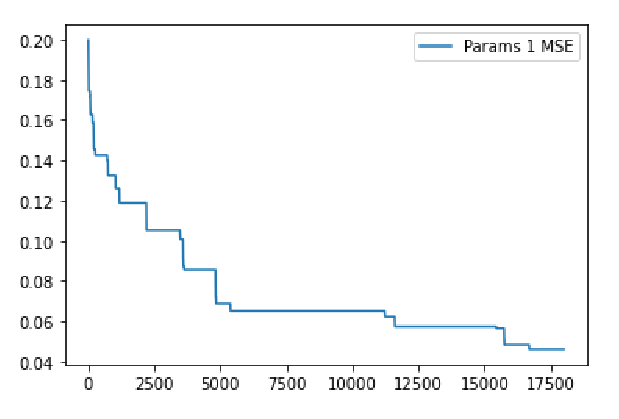
\includegraphics{01}
\begin{center}
Рисунок 1. Результаты работы программы.
\par\end{center}

На данном рисунке представлено изменение среднеквадратичной ошибки
лучшей нейронной сети в процессе работы сети. За 18000 поколений среднеквадратичная
ошибка уменьшилась до значения 0.04628. Таким образом алгоритм обучается,
однако имеет крайне низкую производительность, расчёт занял около
16 часов. Однако следует учитывать, что использовались большие размеры
популяций.

\subsection{Датасет glass1}

Используем несколько вариантов параметров:
\begin{enumerate}
\item размер популяции комбинаций нейронов: 50 для всех вариантов
\item размер популяции нейронов: 1000 для всех вариантов
\item размер скрытого слоя: 5, 5, 25, 25
\item количество соединений на нейрон: 4, 8, 4, 8
\end{enumerate}
Алгоритм инициализируется значениями от -1 до 1. 

Результат представлен на рисунке 2.

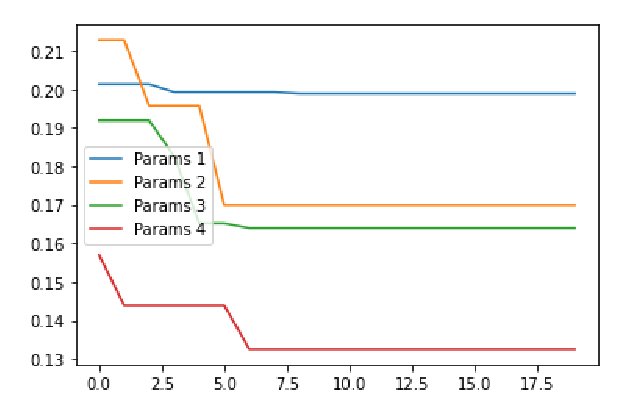
\includegraphics{02}
\begin{center}
Рисунок 2. Результаты работы программы.
\par\end{center}

На данном рисунке представлено изменение среднеквадратичной ошибки
лучших сетей для каждого из набора параметров. Алгоритмы запускались
на 20 поколений. По результатам видно, что при увеличение размера
скрытого слоя увеличивается точность алгоритма. Кроме того видно,
что увеличение количества соединений так же увеличивает точность алгоритма.

\section{Вывод}

В результате выполнения индивидуального задания был реализован нейроэволюционный
алгоритм SANE. Были проанализированы результаты и показано, что алгоритм
решает задачу.
\end{document}
